\documentclass[tikz,border=2pt]{standalone}
\usepackage{tikz}
\usetikzlibrary{positioning}
\begin{document}
% Namikawa--Ueno type: VII^*
% Target MRNC type: 8^{5,7,4}
% Adapted from Tim Dokchitser picture: 8^{5,7,4}
% Parameter substitution: (none)
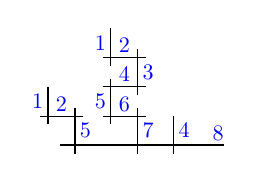
\begin{tikzpicture}[xscale=0.57,yscale=0.62]
\draw[thick,shorten >=2] (4/15,0)--(121/30,0) node[inner sep=2pt,blue,above left,scale=0.8] {8};
\draw[shorten <=-3pt, shorten >=-3pt] (3/5,0)--node[inner sep=2pt,scale=0.8,blue,right] {5} (3/5,3/5);
\draw[shorten <=-3pt, shorten >=-3pt] (3/5,3/5)--node[inner sep=2pt,scale=0.8,blue,above] {2} (0,3/5);
\draw[shorten <=-3pt] (0,3/5)--node[inner sep=2pt,scale=0.8,blue,left] {1} (0,6/5);
\draw[shorten <=-3pt, shorten >=-3pt] (2,0)--node[inner sep=2pt,scale=0.8,blue,right] {7} (2,3/5);
\draw[shorten <=-3pt, shorten >=-3pt] (2,3/5)--node[inner sep=2pt,scale=0.8,blue,above] {6} (7/5,3/5);
\draw[shorten <=-3pt, shorten >=-3pt] (7/5,3/5)--node[inner sep=2pt,scale=0.8,blue,left] {5} (7/5,6/5);
\draw[shorten <=-3pt, shorten >=-3pt] (7/5,6/5)--node[inner sep=2pt,scale=0.8,blue,above] {4} (2,6/5);
\draw[shorten <=-3pt, shorten >=-3pt] (2,6/5)--node[inner sep=2pt,scale=0.8,blue,right] {3} (2,9/5);
\draw[shorten <=-3pt, shorten >=-3pt] (2,9/5)--node[inner sep=2pt,scale=0.8,blue,above] {2} (7/5,9/5);
\draw[shorten <=-3pt] (7/5,9/5)--node[inner sep=2pt,scale=0.8,blue,left] {1} (7/5,12/5);
\draw[shorten <=-3pt] (14/5,0)--node[inner sep=2pt,scale=0.8,blue,right] {4} (14/5,3/5);
\end{tikzpicture}
\end{document}
